
\section{Bineado de eventos}

		
	Fase $\phi$ : $288(60)^o$  \\
	Amplitud $a$: 0.002(2) \footnote{Sí, el error es del 100\% para el ajuste.}  	 \\
		


\begin{figure}[H]
	\centering
	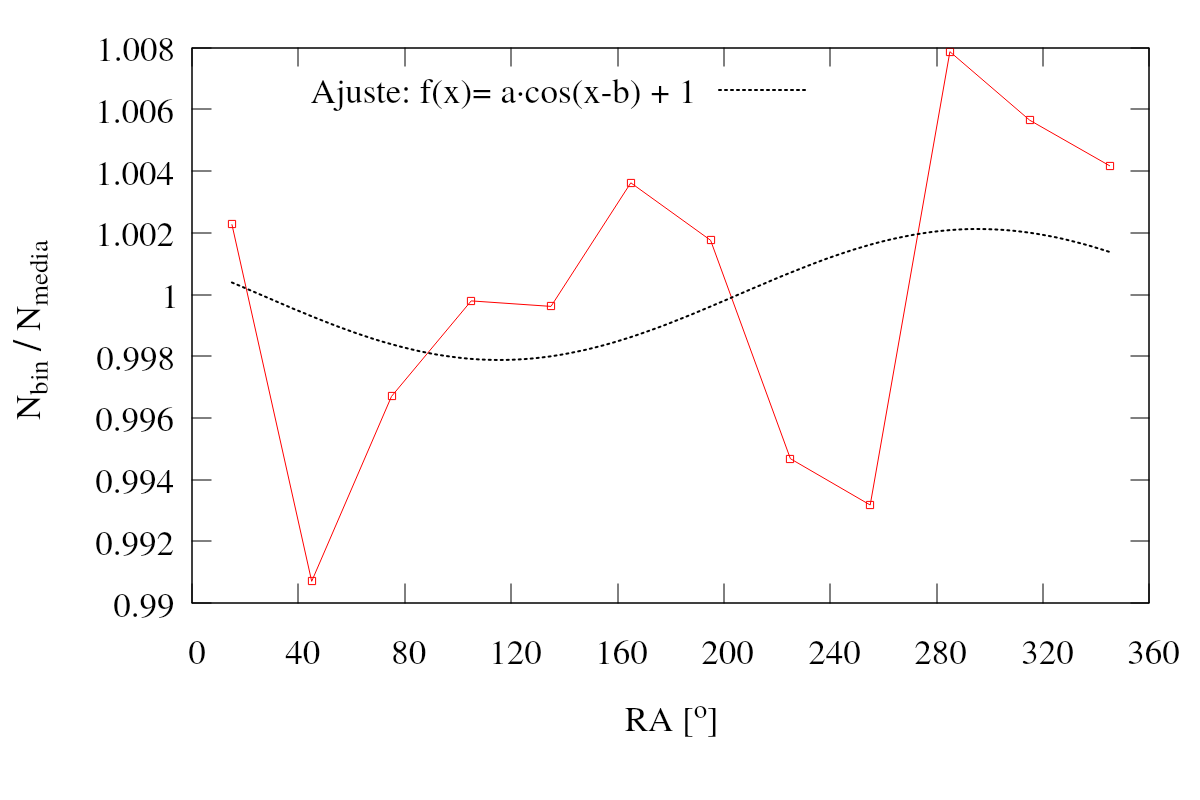
\includegraphics[width=0.95\textwidth]{bineado_eventos_herald_por_RA.png}
	\caption{caption}
\end{figure}

\section{Pesos de los eventos}

			Siderea:
				Con la hora local: Le agregué 2 porque esa es la hora SIDEREA del cenit, así están en fase.
				Con la ascensión recta:
		
		
		
		\begin{figure}[H]
			\centering
			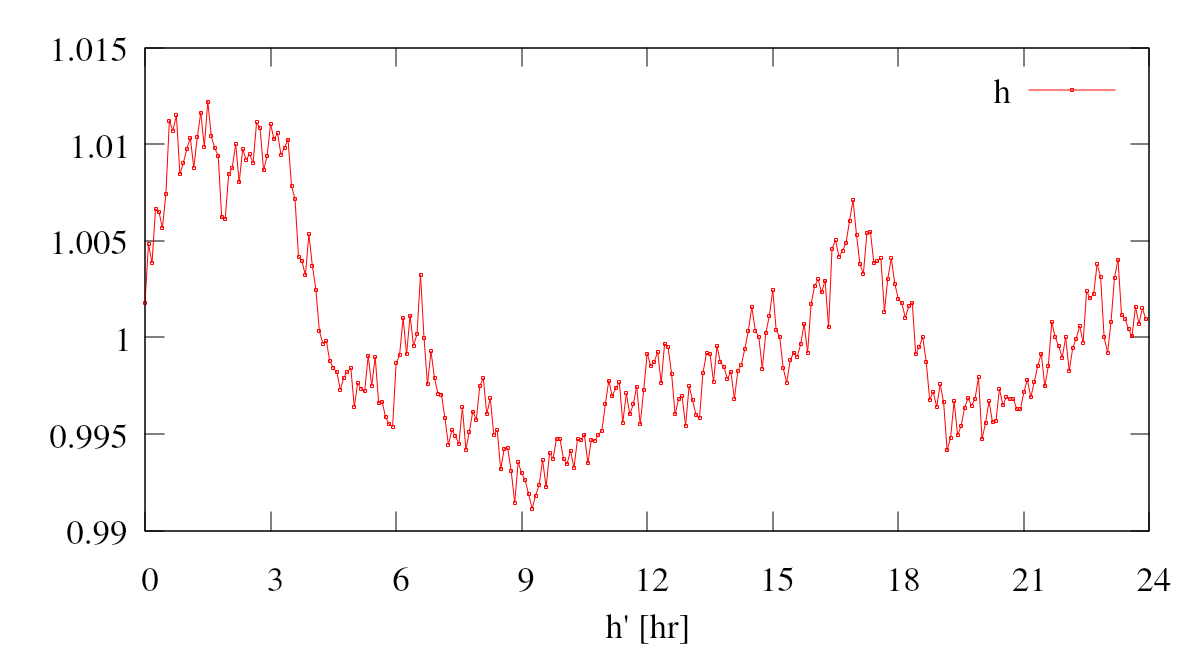
\includegraphics[width=0.65\textwidth]{eventos_hora_local.png}
			\caption{Usando el valor $h$ para calcular los pesos.}
		\end{figure}
		
		
		\begin{figure}[H]
			\centering
			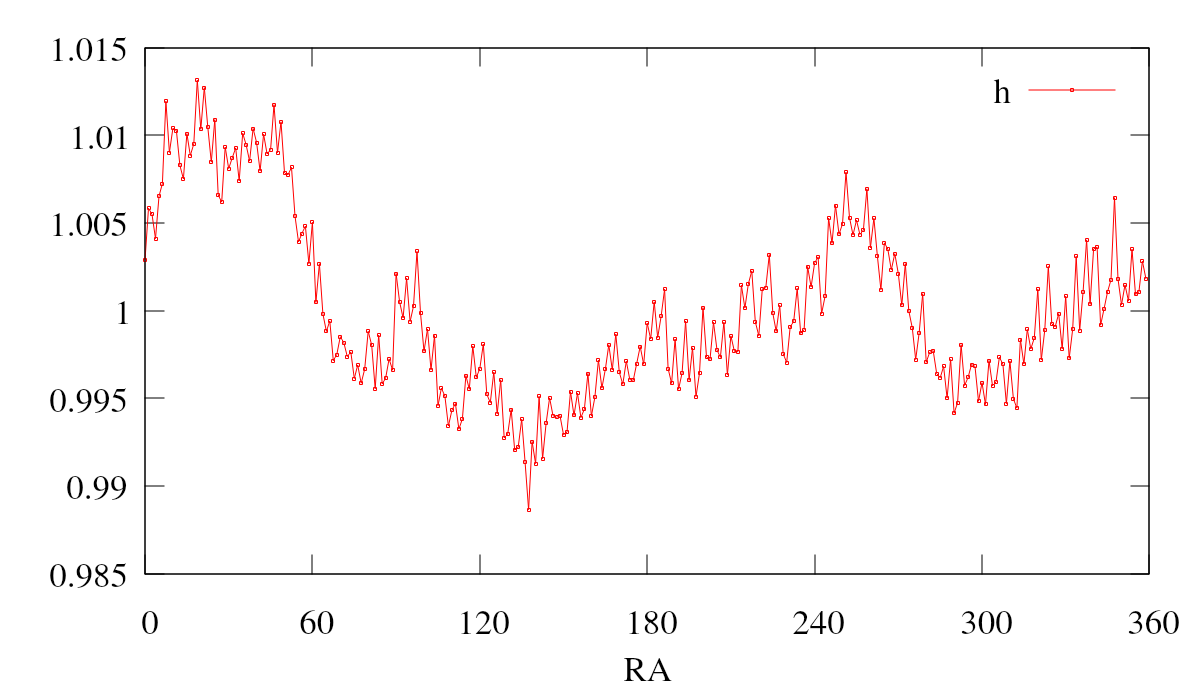
\includegraphics[width=0.65\textwidth]{eventos_RA.png}
			\caption{Usando la ascensión recta para calcular los pesos.}
		\end{figure}
		

\section{Grafico de la anisotropia}

		
		Dataset data:
		
		
		\begin{enumerate}
			\item Energía entre  [1 EeV , 2 EeV)
			\item Rango de tiempo:
			\begin{itemize}
				\item[-] Inicial:1388577600 (Thursday, 1 January 2014 12:00:00 GMT)
				\item[-] Final: 1577880000  (Thursday, 1 January 2020 12:00:00 GMT)
			\end{itemize}
			\item Ángulo cenital $\theta < 60^o$
			\item 6T5
			\item $ib=1$ Bad period flag. Un valor de 1 indica un buen periodo
			\item Número de eventos: $1\,081\,844$
		\end{enumerate}
		
		
		
		Tabla comparando:
		
		\begin{table}[H]
		\centering
		
		\begin{tabular}{c|c|c}
					& Solar 		& Siderea\\ \hline
		Fase $\phi$ & 30(7) 	    & 356(5) 			\\
		Amplitud $a$& 0.0047(6)	    &0.0038(6)			\\
		\end{tabular}
		
		\end{table}
		
		
		
		\begin{figure}[H]
			\centering
			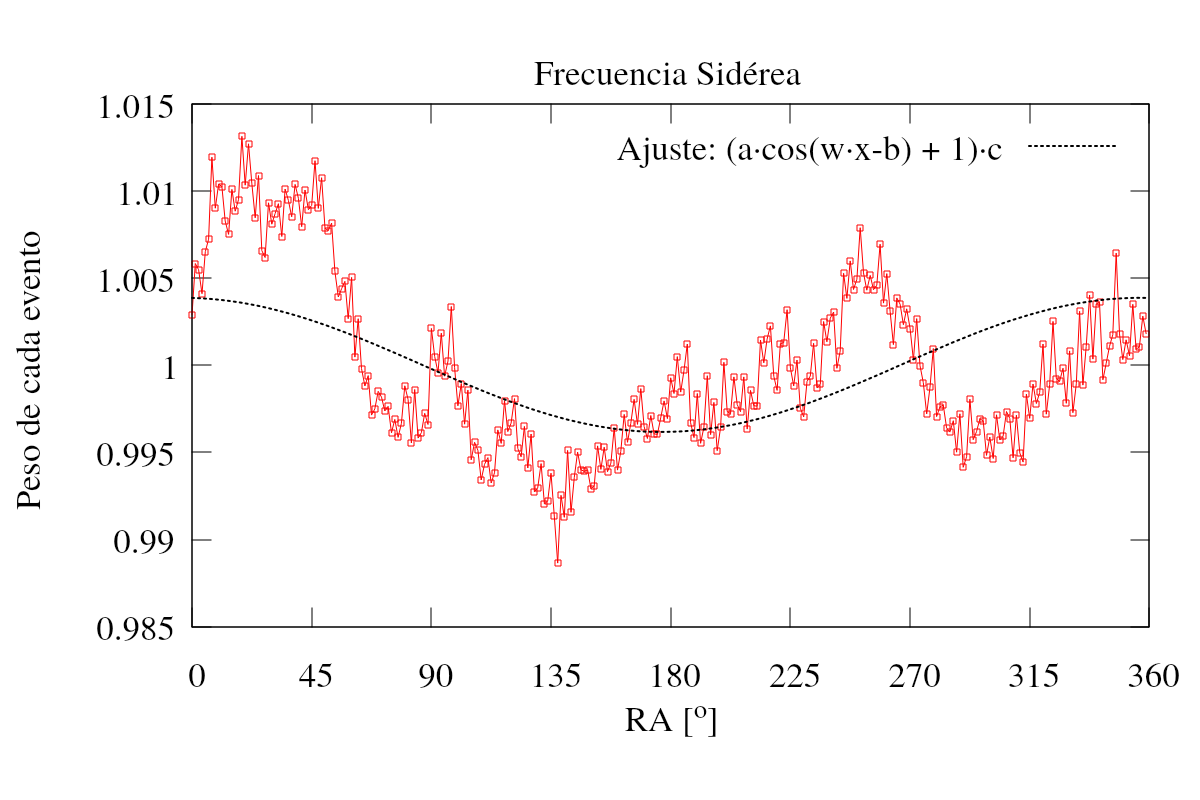
\includegraphics[width=0.95\textwidth]{eventos_RA_ajuste_cos.png}
			\caption{caption}
		\end{figure}
		
		
		
		
		
		\begin{figure}[H]
			\centering
			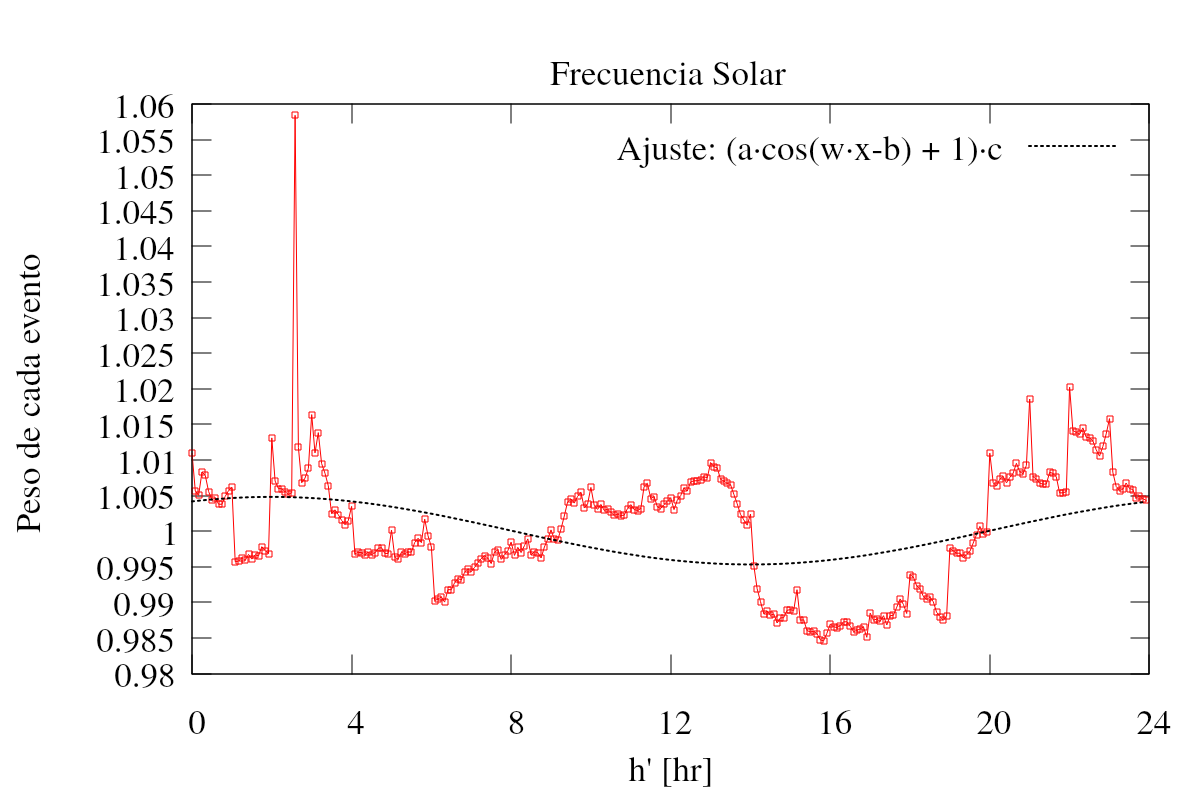
\includegraphics[width=0.95\textwidth]{eventos_hora_local_ajuste_cos.png}
			\caption{caption}
		\end{figure}
		
		Graficos comparando:
		
		\begin{figure}[H]
			\centering
			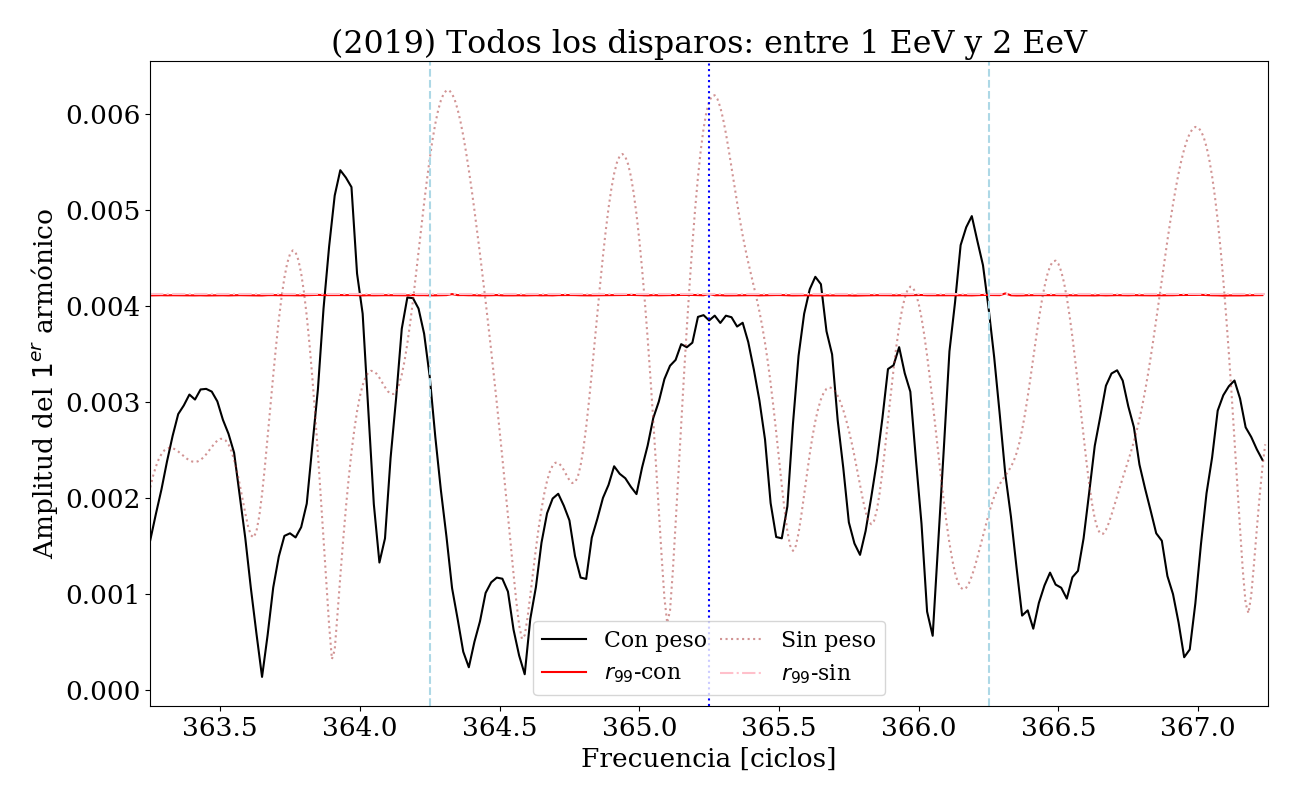
\includegraphics[width=0.95\textwidth]{pesos_sin_con_1_2_EeV.png}
			\caption{Anisotropía en función de la frecuencia, se comparan los análisis sin los pesos y con los pesos de los hexagonos}
		\end{figure}
		
		
		\begin{table}
		\centering
		\begin{tabular}{c|c|c}
					& Solar (sin peso)		& Siderea (sin peso)  \\ \hline
		Fase $\phi$ & 224.681	    		& 335.104			\\
		Amplitud $r$& 0.00706339	    	&0.00404635			\\
		\end{tabular}
		
		\end{table}
		
		\begin{table}
		\centering
		\begin{tabular}{c|c|c}
					& Solar (con peso)		& Siderea (con peso)  \\ \hline
		Fase $\phi$ & 286.567	    	& 335.104			\\
		Amplitud $r$& 0.00383264	    &0.00404635			\\
		\end{tabular}
		\end{table}
		
		
		